\section{Multiple Predictor Model with Ads and Price}
\subsection{Call}
\[
	lm(formula = sales\_units \sim TV\_ads + online\_ads + print\_ads + price, data = sat.df)
\]
\subsection{Statsmodels OLS Results}
\begin{table}[htb!]
\centering
\begin{tabular}{lrrrr}
	\toprule
	Coefficients & Estimate & Std. Error & t value & Pr(>|t|) \\
	\midrule
	(Intercept) & 1296.6590 & 188.4731 & 6.880 & 1.67e-10 *** \\
	tv\_ads & 7.4959 & 0.7697 & 9.738 & < 2e-16 *** \\
	online\_ads & 320.2256 & 8.2327 & 38.897 & < 2e-16 *** \\
	print\_ads & 1134.2760 & 149.4127 & 7.592 & 3.54e-12 *** \\
	price & -15.5628 & 0.5332 & -29.189 & < 2e-16 *** \\
	\bottomrule
\end{tabular}
\begin{tabular}{l}
Significance codes:  0 ‘***’ 0.001 ‘**’ 0.01 ‘*’ 0.05 ‘.’ 0.1 ‘ ’ 1 \\
Residual standard error: 88.51 on 145 degrees of freedom \\
Multiple R-squared:  0.9504, Adjusted R-squared:  0.949 \\
F-statistic: 694.3 on 4 and 145 DF, p-value: < 2.2e-16 \\
\end{tabular}
\caption{\label{tab:table-name}Coefficients.}
\end{table}
\begin{table}[htb!]
\centering
\begin{tabular}{rrrrr}
	\toprule
	Min & 1Q & Media & 3Q & Max \\
	\midrule
	-262.83 & -48.52 & 10.73 & 66.45 & 202.31 \\
	\bottomrule
\end{tabular}
\caption{\label{tab:table-name}Residuals.}
\end{table}
\pagebreak
\section{Figures}
\begin{figure}[htb!]
\centering
  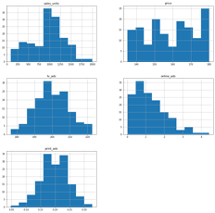
\includegraphics[width=0.6\textwidth]{distribution}
  \caption{Unscaled distribution of independent variables}
\end{figure}

\begin{figure}[htb!]
\centering
  
\includegraphics[width=0.6\textwidth]{multicollinearity}
  \caption{Independent variable multicollinearity heatmap}
\end{figure}

\begin{figure}[htb!]
\centering
  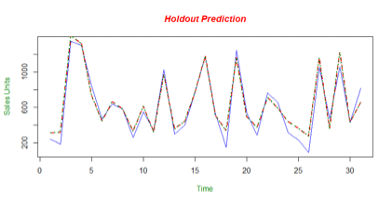
\includegraphics[width=0.8\textwidth]{holdout}
  \caption{Holdout Predictions of the OLS model}
\end{figure}

\begin{figure}[htb!]
\centering
  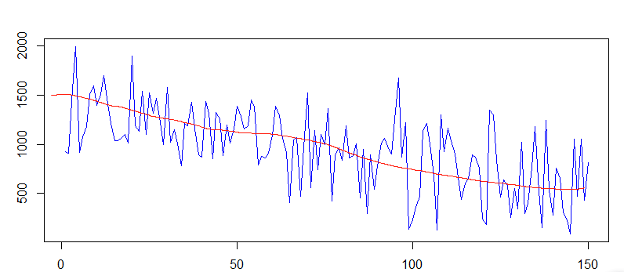
\includegraphics[width=0.8\textwidth]{volume_over_time}
  \caption{Volume of Sales Units Over Time by Month}
\end{figure}

